Two simplified test cases were constructed, both using three demand and three supply sites with
demand varying over 5 years. In the first case the optimal solution was for the closest site to provide
power, in the second this was the case for all but the final year, when it became optimal for one station
to provide all power due to cost increases for the other stations.

Both methods converged on the optimal solutions. These results are conveyed 
below in table \ref{tab:baseline_performance}. Figure \ref{fig:base_cases} shows 
the base case solutions found, which correspond to the designed optimal setups.
The demand fluctuation are not displayed, but the thickness of the lines indicates
the proportion of total energy supplied to each site 
of the total energy over all time periods.
\begin{figure}[H]
    \centering
    \begin{subfigure}[b]{0.45\textwidth}
        \centering
        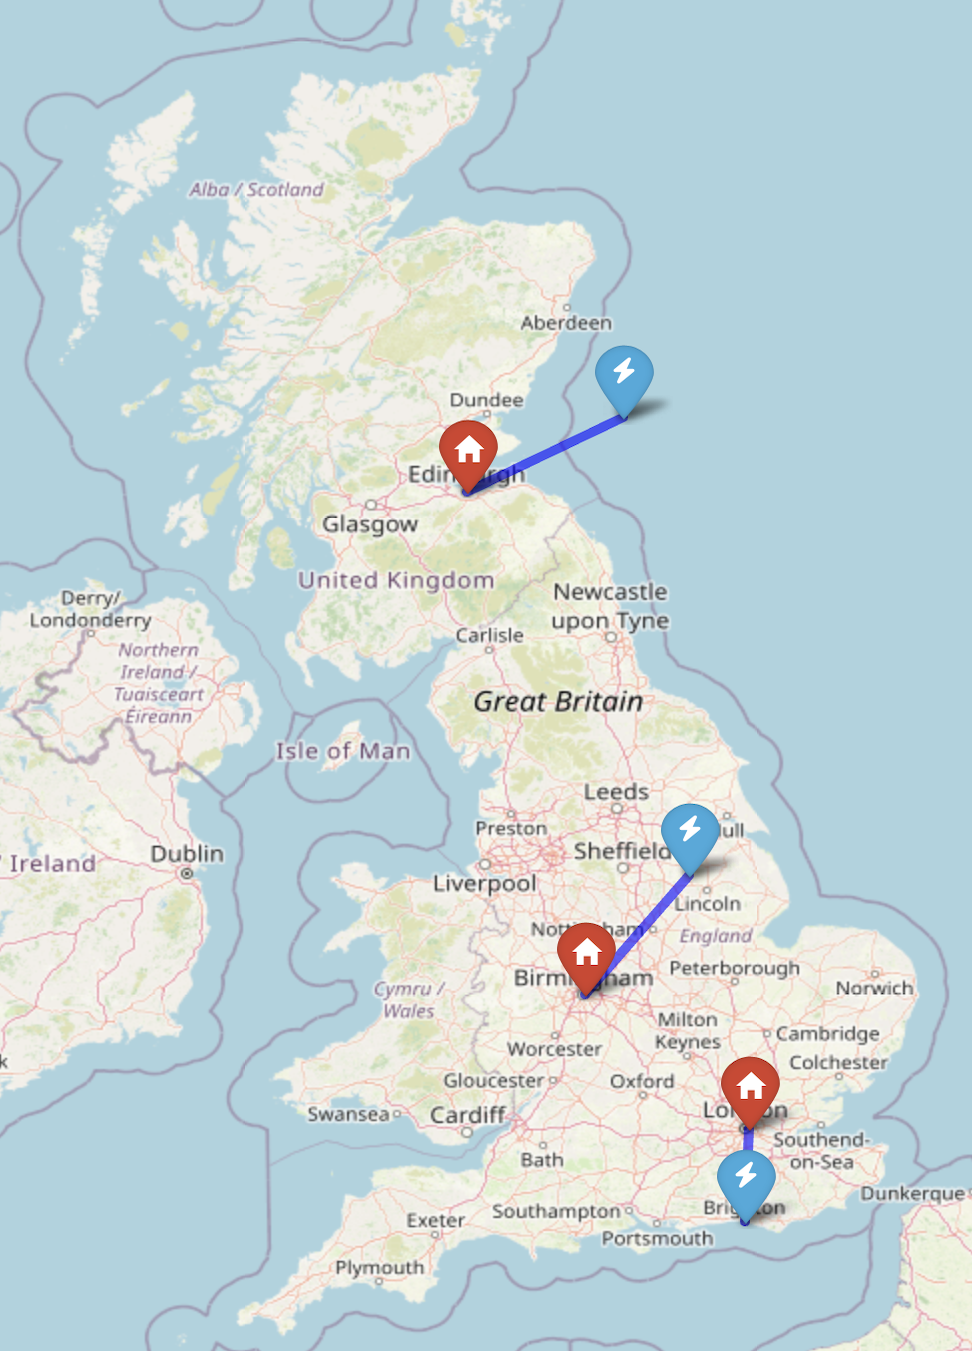
\includegraphics[width=\textwidth]{figures/base_case_1.png}
        \caption{Base Case 1: 3 demand sites each with one optimal supply site over entire time horizon}
        \label{fig:base_case_1}
    \end{subfigure}
    \hfill
    \begin{subfigure}[b]{0.45\textwidth}
        \centering  
        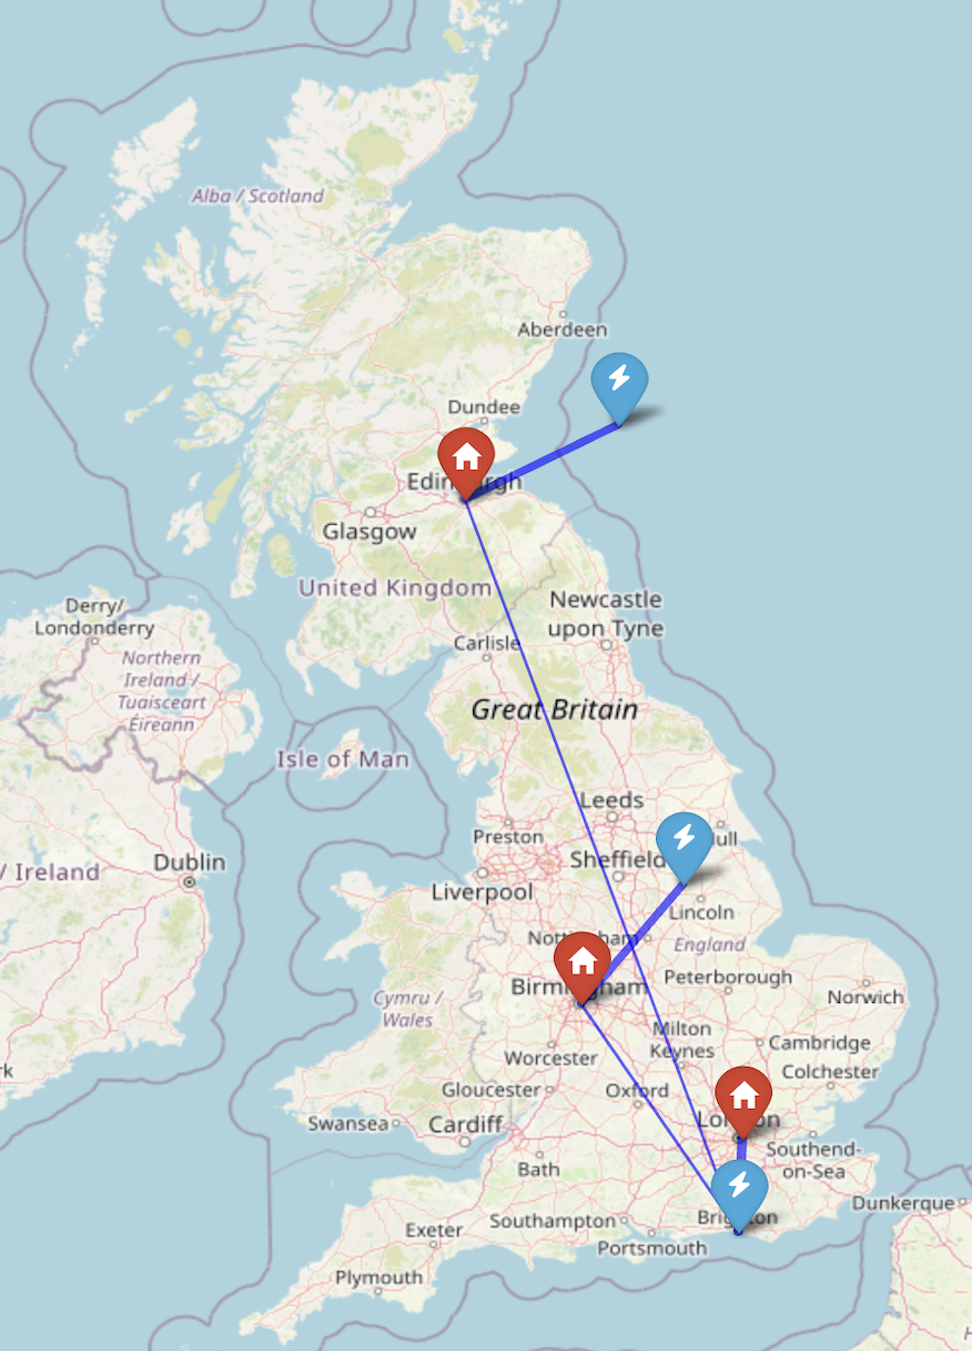
\includegraphics[width=\textwidth]{figures/base_case_2.png}
        \caption{Base Case 2: 3 demand sites each with one optimal supply site over entire time horizon
        except for final timestep}
        \label{fig:base_case_2}
    \end{subfigure}
    \caption{Base Case results compared}
    \label{fig:base_cases}
\end{figure}

\begin{table}[h]
    \centering
    \caption{Performance Comparison of LR Heuristic and to ESLP}
    \label{tab:baseline_performance}
    \renewcommand{\arraystretch}{1.2}
    \setlength{\tabcolsep}{10pt} % Adjust column spacing
    
    \begin{tabular}{l ccc c}
        \toprule
        \textbf{Test Case} & \multicolumn{3}{c}{\textbf{LR Heuristic}} & \textbf{ESLP} \\
        \cmidrule(lr){2-4} \cmidrule(lr){5-5}
         & \textbf{Time (s)} & \textbf{Gap} & \textbf{Iterations} & \textbf{Time (s)} \\
        \midrule
        1 & 0.12 & 0.0 & 1 & 0.14 \\
        2 & 0.14 & 0.0 & 2 & 0.16 \\
        \bottomrule
    \end{tabular}
\end{table}




